%%%%%%%%%%%%%%%%%%%%%%%%%%%%%%%%%%%%%%%%%%%%%%%%%%%%%%%%%%%%%%%%%%%%%%
%    
% Written by   Colin Morris                              
%              Department of Mechanical Engineering
%              University of Washington, Seattle, WA                            
% 
% Title:       Cooperative pHRI
% Created:     October 24, 2017                 
%  
%%%%%%%%%%%%%%%%%%%%%%%%%%%%%%%%%%%%%%%%%%%%%%%%%%%%%%%%%%%%%%%%%%%%%%

\documentclass[conference]{IEEEtran}
\IEEEoverridecommandlockouts
\usepackage{cite}
\usepackage{amsmath,amssymb,amsfonts}
\usepackage{algorithmic}
\usepackage{graphicx}
\usepackage{textcomp}
\usepackage{longtable}
\usepackage[utf8]{inputenc}
\usepackage{longtable}
\def\BibTeX{{\rm B\kern-.05em{\sc i\kern-.025em b}\kern-.08em
    T\kern-.1667em\lower.7ex\hbox{E}\kern-.125emX}}
    
\begin{document}
\title{Towards Seamless Interaction in \\ Cooperative pHRI} 
\author{Colin Morris}
\maketitle

\section{Problem Statement} 
\hspace{5mm}
We are interested in the situation in which a human and a robot interact in a world-space $\mathcal{W}$ through a deterministic dynamical system $f : \mathcal{X}_h \times \mathcal{X}_r \rightarrow \mathcal{U}_{sys}$. For example, consider the simple case in which the human and robot are tied together through a spring where $\mathcal{W}\subset\mathbb{R}^2$. 

\begin{equation*}
\begin{bmatrix} u_{1,sys}(t)\\u_{2,sys}(t) \end{bmatrix} = 
\begin{bmatrix} k_1&0\\0&k_2 \end{bmatrix}
\begin{bmatrix} x_{1,h}(t) - x_{1,r}(t) \\x_{2,h}(t) - x_{2,r}(t) \end{bmatrix}
\end{equation*}

The magnitude of the net interaction force $|u_{sys}|$ between the human and the robot is thus the euclidean norm $||u_{sys}||_{_2}$. 
We assume that the human and robot live in the same physical world-space $\mathcal{W}$, begin with the same initial states $x(t_0)$ , and wish to move together to a final goal state $x_g \equiv x(t_f) $ . It is assumed that the final state $x_g$ is deterministic, and is known to both the robot and the human a priori. It is also assumed that all current human and robot \textit{physical} states ($x_h \in \mathcal{X}_h$ , $x_r \in \mathcal{X}_r$) are deterministic, yet their actions ($a_h \in \mathcal{A}_h$ , $a_r \in \mathcal{A}_r$) to future states are stochastic. \\

To quantify the \textit{degree of cooperation} between the human and robot, a performance metric is defined:
 
\begin{equation}
C^{\pi_h,\pi_r} = \int_{t_0}^{t_f} \lVert u_{sys}(t)\rVert_{_2}  dt
\end{equation}

This performance metric is a measure of how much cumulative momentum transfer occurs between the robot and the human throughout the duration of the interaction --- recall that the equation for momentum change is: $\Delta p = \int_T u(t)dt$. We wish to minimize the total shift in momentum between human and robot (and perhaps also minimize the task duration $t_f$). Consequently, we seek an policy $\pi_r^*(a|s)$ which minimizes $C^{\pi_h,\pi_r}$, by influencing and/or being influenced by $\pi_h(a|s)$ through the dynamics $f(\cdot)$.

\hspace{5mm}
\subsection{Problem 1: Identical World-Space Perception}
\hspace{5mm}

A baseline interaction is pictorialized in figure 1. We define the world-space \textit{percieved} by the human and robot as $\mathcal{W}_h$ and $\mathcal{W}_r$ respectively. In this scenario, we assume that the human and robot perfectly perceive the world-space, such that  $ \mathcal{W}_r = \mathcal{W}_h = \mathcal{W}$. The world-space may contain obstacles $\mathcal{C} \subset \mathcal{W}$ in which the human and robot must cooperatively avoid to reach $x_g$. Any ambiguity between the chosen paths $x_h(t)$ and $x_r(t)$ must be cooperatively resolved, else collisions may occur. Problem 1 requires inferences on the human latent states of: (1) intent (future actions), (2) expertise, and (3) adaptability. 

\begin{figure}[h!]
\begin{center}
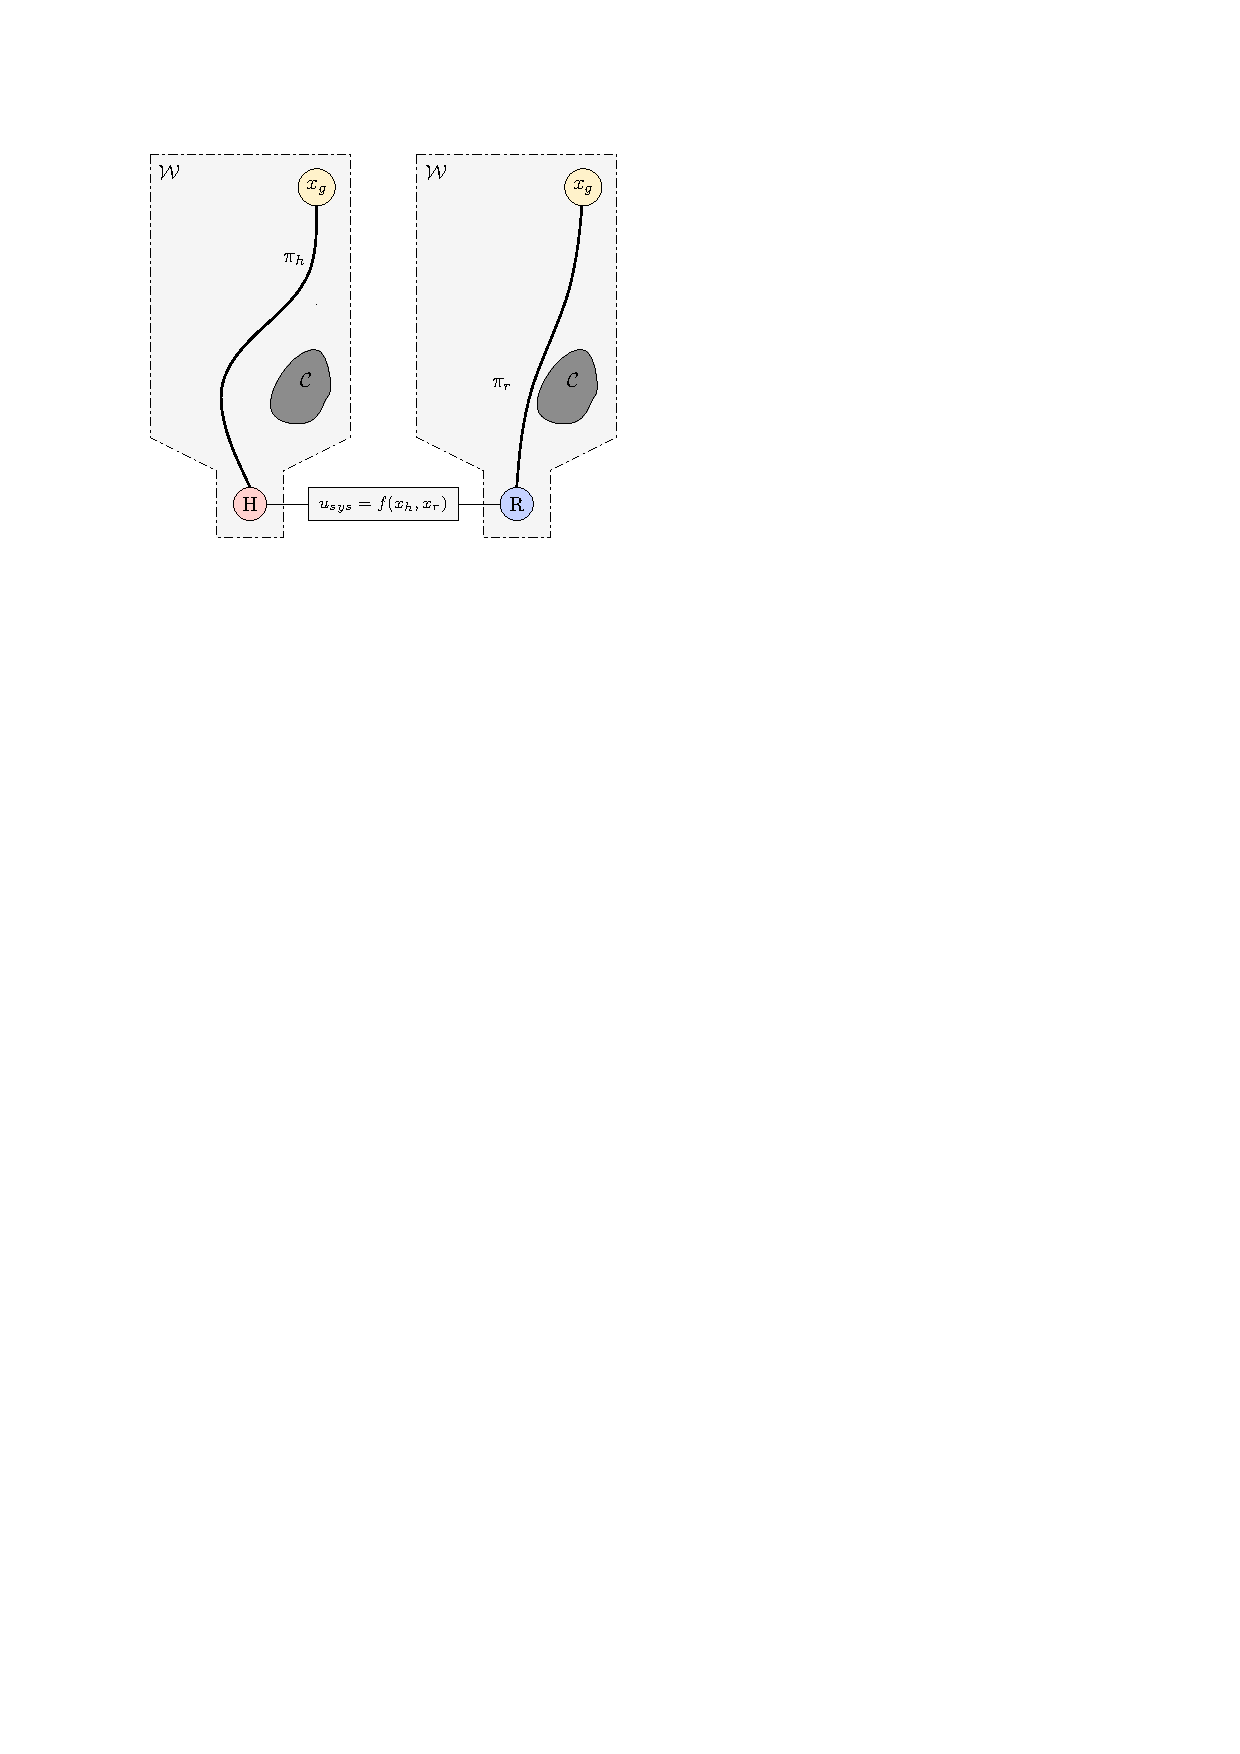
\includegraphics{diag1.pdf}
  \caption{Human and robot agents are tied together through the dynamical system $f(\cdot)$ and wish to move to location $x_g$. The human and robot live in the same world-space, and have identical perceptions of the world space. This is to say, both agents are aware of all obstacles.}
\end{center}
\end{figure}
\subsection{Problem 2: Variant World-Space Perception}

\hspace{5mm}
Now we assume a more generalized scenario in which the perceived human and robot world-spaces are different: $\mathcal{W}_r \neq \mathcal{W}_h$. This results in three possible scenarios, which are summarized in the table below. In scenario 1, the human cannot see all obstacles, but the robot can. In scenario 2, the opposite it true. In scenario 3, there are obstacles that the human can see and the robot cannot, while there are also obstacles that the robot can see but the human cannot (refer to figure 2). Additionally, we impose a world-space constraint $\mathcal{C} = \mathcal{C}_h \cup \mathcal{C}_r$ , which prevents any obstacle from being simultaneously unknown to both agents. \\

\begin{center}
\begin{tabular}{c | c c c c c c}
\hline
\# & $\mathcal{W}_h$                  & $\mathcal{W}_r$               &               & $\mathcal{C}_h$                  & $\mathcal{C}_r$ \\
\hline
\\
1 & $\mathcal{W}_h \neq \mathcal{W}$ & $\mathcal{W}_r = \mathcal{W}$ & $\rightarrow$ & $\mathcal{C}_h \neq \mathcal{C}$ & $\mathcal{C}_r = \mathcal{C}$  \\
\\
2 & $\mathcal{W}_h = \mathcal{W}$ & $\mathcal{W}_r \neq \mathcal{W}$ & $\rightarrow$ & $\mathcal{C}_h = \mathcal{C}$ & $\mathcal{C}_r \neq \mathcal{C}$  \\
\\
3 & $\mathcal{W}_h \neq \mathcal{W}$ & $\mathcal{W}_r \neq \mathcal{W}$ & $\rightarrow$ & $\mathcal{C}_h \neq \mathcal{C}$ & $\mathcal{C}_r \neq \mathcal{C}$   \\
\end{tabular}
\end{center} 

\begin{figure}[h!]
\begin{center}
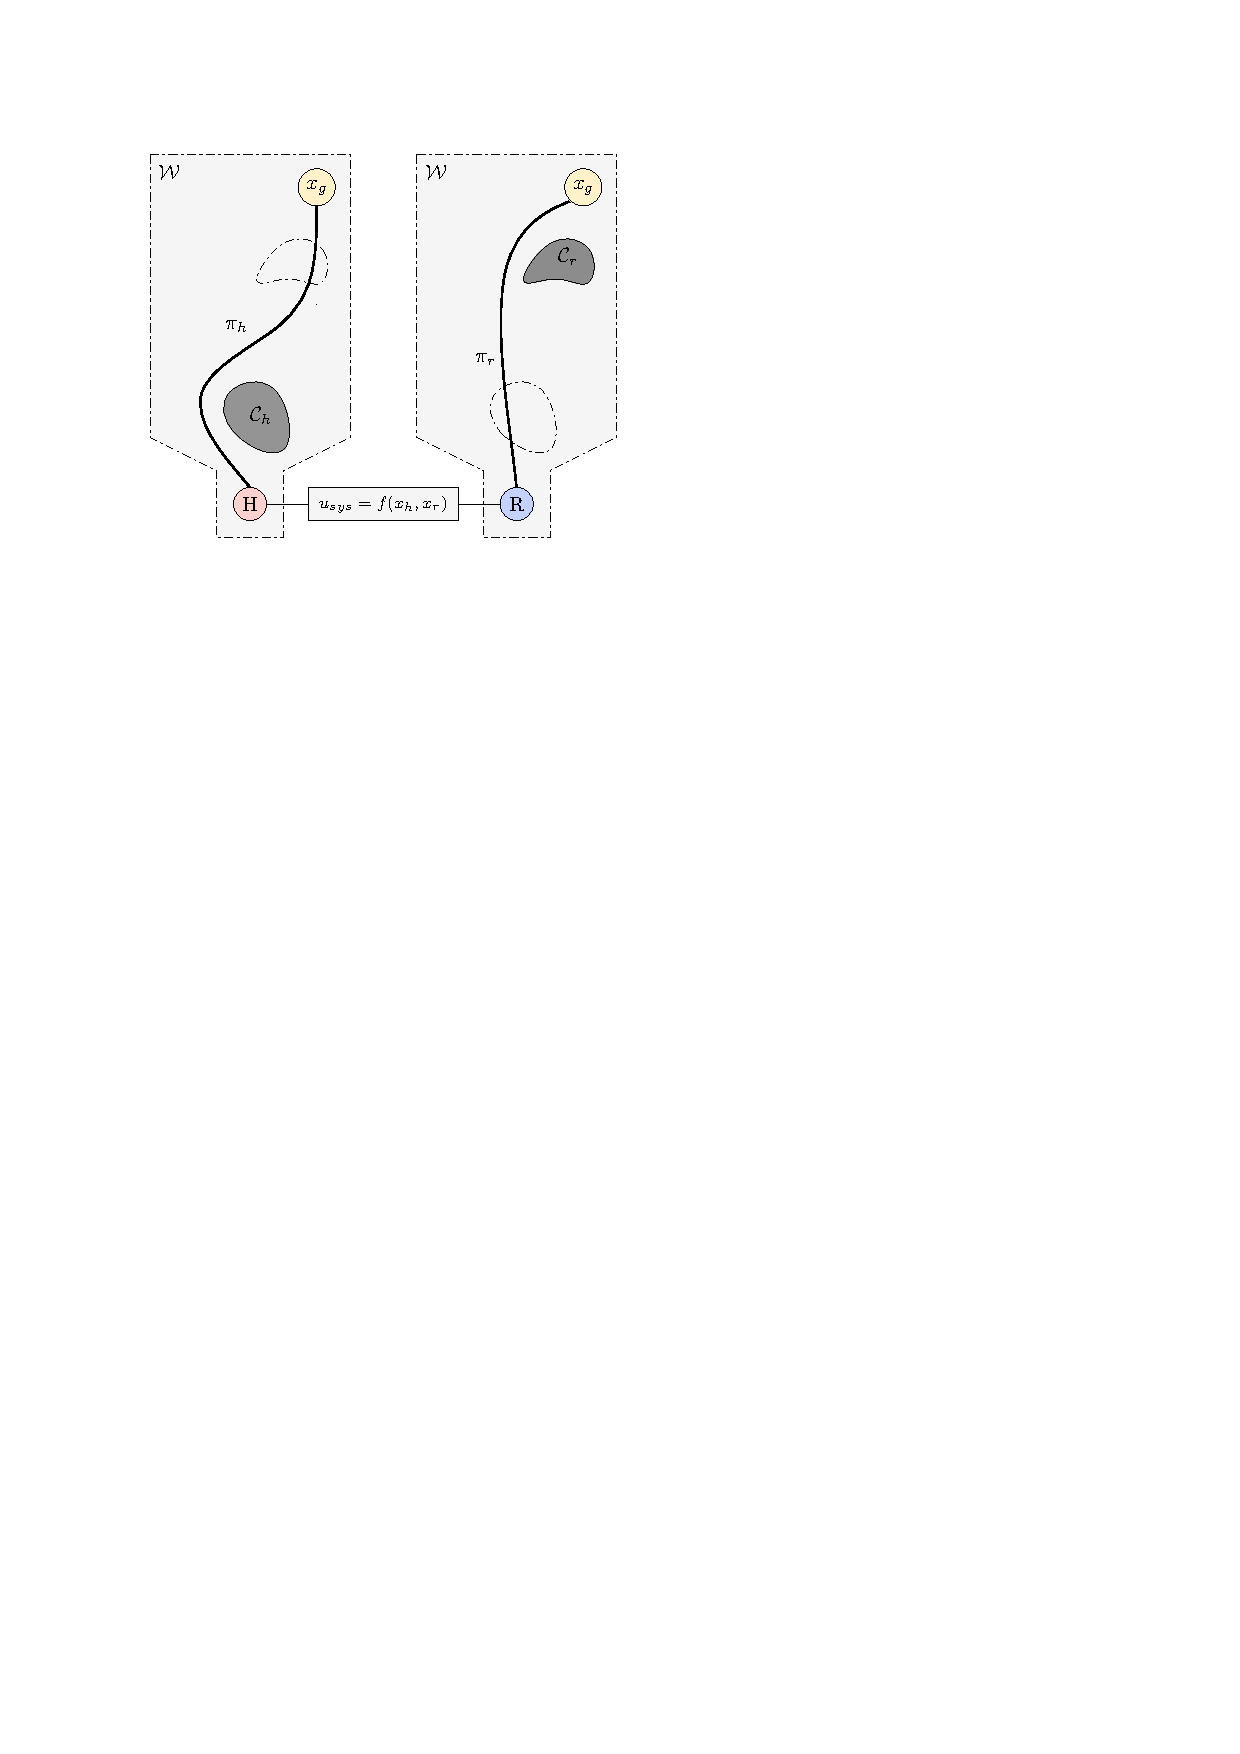
\includegraphics{diag2.pdf}
  \caption{ The human and robot live in the same world-space,but now have conflicting perceptions of the world-space. This figure illustrates situation 3, in which both the human and robot do not percieve all obstacles in world-space.}
\end{center}
\end{figure}
\hspace{2cm} 

The imposed constraint that $\mathcal{W}_r \neq \mathcal{W}_h$ introduces interesting challenges. In scenario 1, the robot must find a way to communicate information about the unknown obstacles \textit{to} the human \textit{through} the dynamical system. This should be done in a matter which minimizes $C^{\pi_h,\pi_r}$ with respect to control $u_{sys}$, time $t_f$, or both. If both $u_{sys}$ and time $t_f$ are to be Pareto-optimized, one human may prefer a particular location on the Pareto front over another human. This, in itself, makes for an interesting problem. 

In scenario 2, one of two things must happen: either the human must find a way to efficiently communicate to the robot about unperceived obstacles, or the robot must find a way to efficiently infer where the obstacles are based on human latent states. One core question I would eventually like to pursue is: how much better (if at all) can a robot make inferences about unperceived obstacles by making inferences from human eye gaze. 
Note: scenario 3 is a combination of both scenarios 1 and 2. 

\section{Prior Work} 

\end{document}